\documentclass[11pt]{article}

\author{Math 123}
\date{Due February 3, 2023 by 5pm} 
\title{Homework 1}

\usepackage{graphicx,xypic}
\usepackage{amsthm}
\usepackage{amsmath,amssymb}
\usepackage{amsfonts}
\usepackage{xcolor}
\usepackage[margin=1in]{geometry}
\usepackage[shortlabels]{enumitem}
\newtheorem{problem}{Problem}
\renewcommand*{\proofname}{{\color{blue}Solution}}


\usepackage{fancyhdr}
\pagestyle{fancy}
\rhead{Math 123, Homework 1}

\setlength{\parindent}{0pt}
\setlength{\parskip}{1.25ex}


\begin{document}

\maketitle

% You are required to put your name here:
{\bf\Large Name:} 


\vspace{.3in}
Topics covered: graph, subgraph, cycle, path, vertex degrees, 

Instructions: 
\begin{itemize}
\item This assignment must be submitted on Gradescope by the due date. Gradescope Entry Code: RZ277D. 
\item If you collaborate with other students (which is encouraged!), please mention this near the corresponding problems. 
\item If you are stuck, please ask for help (from me, a TA, a classmate).  
\end{itemize}

\pagebreak 




\begin{problem}
Prove that the graph below is isomorphic to the Petersen graph.\footnote{Hint: label the graph.}
\begin{center}
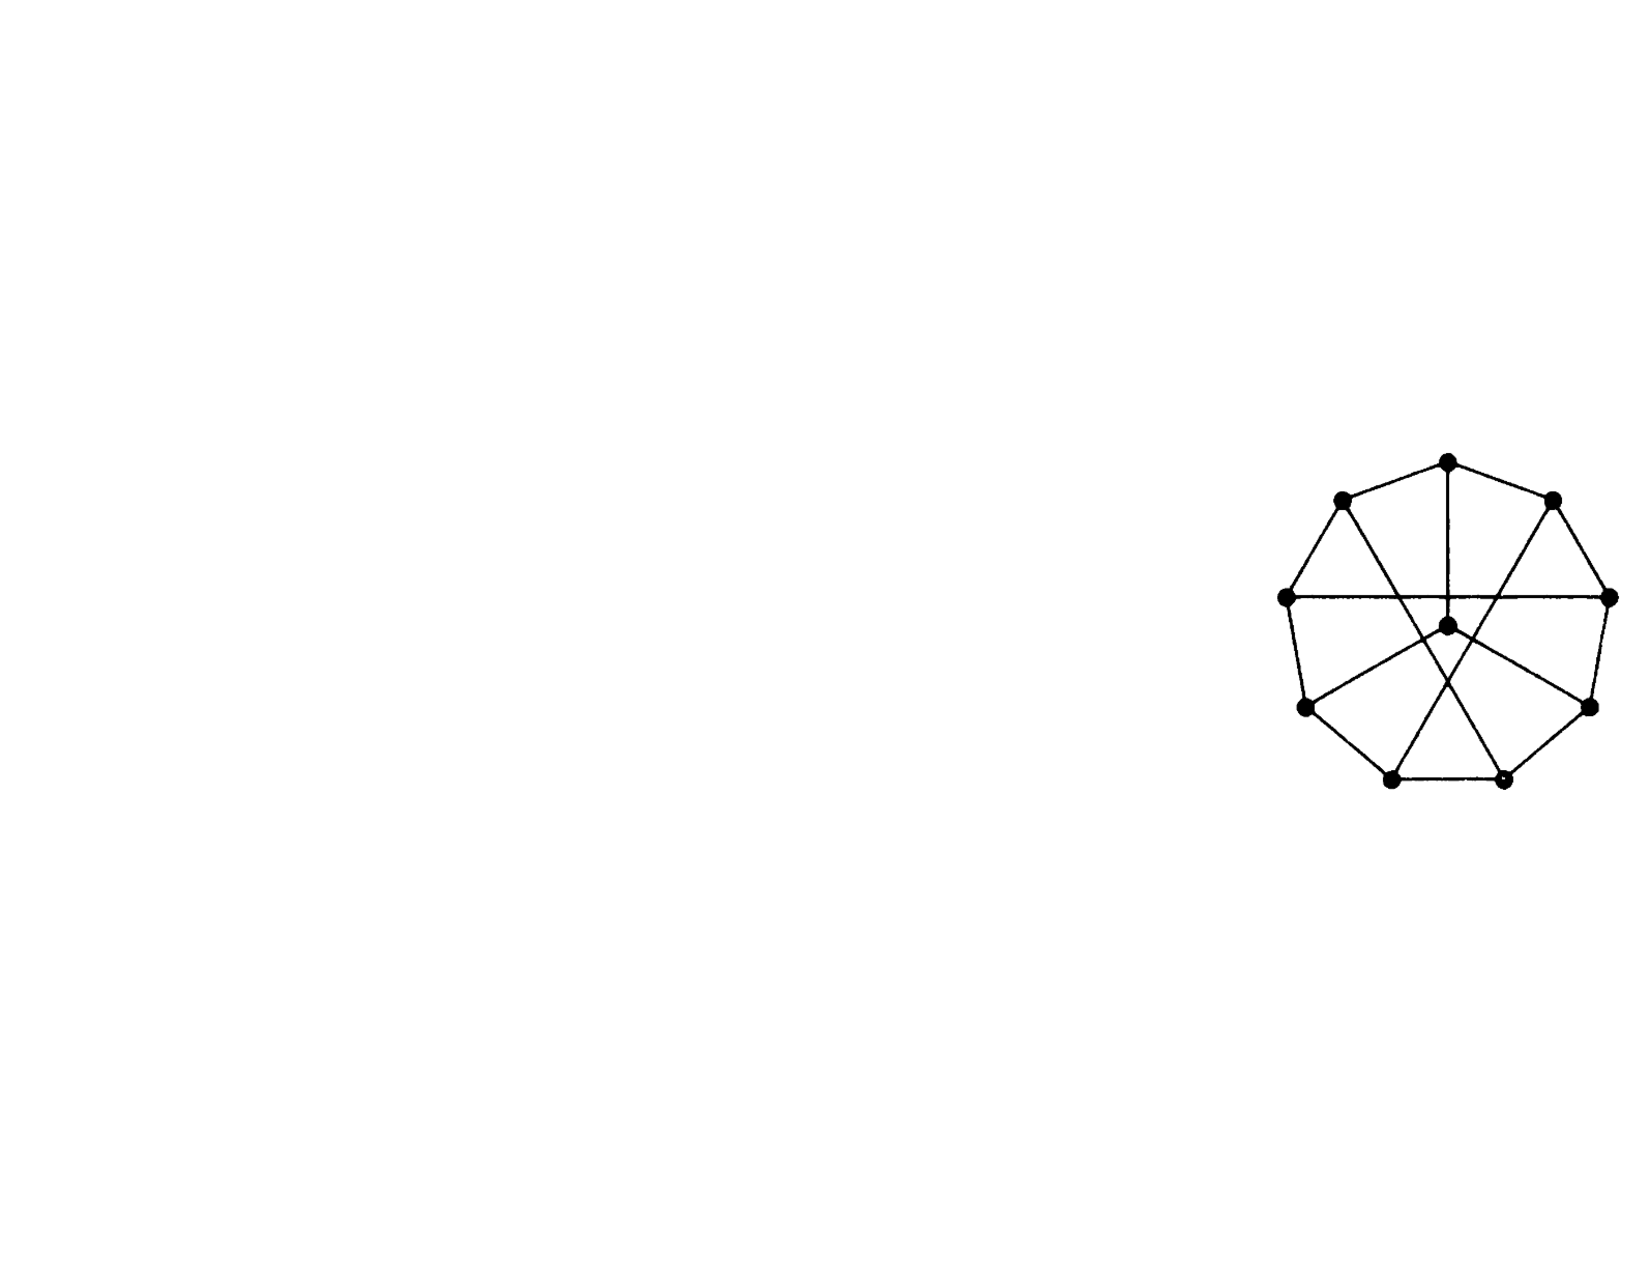
\includegraphics[scale=.4]{petersen.pdf}
\end{center}
\end{problem}

\begin{proof}

\end{proof}


\begin{problem}
How many cycles of length $n$ are there in the complete graph $K_n$?
\end{problem}

\begin{proof}

\end{proof}

\begin{problem}
Define the hypercube graph $Q_k$ as the graph with a vertex for each tuple $(a_1,\ldots,a_k)$ with coordinates $a_i\in\{0,1\}$ and with an edge between $(a_1,\ldots,a_k)$ and $(b_1,\ldots,b_k)$ if they differ in exactly one coordinate.\footnote{Suggestion: Draw $Q_k$ for $k=2$ and $k=3$.} 
\begin{enumerate}[(a)]
\item Prove that two $4$-cycles in $Q_k$ are either disjoint, intersect in a single vertex, or intersect in a single edge.
\item Let $K_{2,3}$ be the complete bipartite graph with $2$ red vertices, $3$ blue vertices, and all possible edges between red and blue vertices. Prove that $K_{2,3}$ is not a subgraph of any hypercube $Q_k$. 
\end{enumerate} 
\end{problem}

\begin{proof}

\end{proof}

\begin{problem}
For a graph $G=(V,E)$, the complement of $G$ is the graph $\bar G=(V,\bar E)$, where $\{u,v\}\in\bar E$ if and only if $\{u,v\}\notin E$. Prove or disprove: If $G$ and $H$ are isomorphic, then the complements $\bar G$ and $\bar H$ are also isomorphic. 
\end{problem}

\begin{proof}

\end{proof}


\begin{problem}\ 
\begin{enumerate}[(a)]
\item Determine the complement of the graphs $P_3$ and $P_4$. (Recall that $P_n$ is the path with $n$ vertices. It has $n-1$ edges.)
\item We say that $G$ is self-complementary if $G$ is isomorphic $\bar G$. Prove that if $G$ is self-complementary with $n$ vertices, then either $n$ is divisible by $4$ or $n-1$ is divisible by $4$. \footnote{Hint: count edges}
\end{enumerate} 
In fact, whenever $n$ or $n-1$ is divisible by $4$, there is a self-complementary graph with $n$ vertices -- see the bonus problem below. 
\end{problem}

\begin{proof}

\end{proof}


\begin{problem}Prove that the Petersen graph has no cycles of length $3$ or $4$. \footnote{Hint: use the definition of Petersen graph given in class.} 
\end{problem}

\begin{proof}

\end{proof}

\begin{problem}[Bonus]
Let $G,H$ be a self-complementary graphs, and assume $G$ has with $4k$ vertices. Construct a self-complementary graph obtained by taking the union of $G$ and $H$ and adding some edges.\footnote{Hint: How does the degree of even/odd vertices of $G$ change after taking the complement?} Deduce that if either $n$ or $n-1$ is divisible by $4$, then there is a self-complementary graph with $n$ vertices. 
\end{problem}

\begin{proof}

\end{proof}


\end{document}